\documentclass{article}

\usepackage[final]{project_nips_style}

% =========================
% Packages
% =========================
\usepackage[utf8]{inputenc}
\usepackage[T1]{fontenc}
\usepackage{hyperref}
\usepackage{url}
\usepackage{booktabs}
\usepackage{amsmath, amsfonts}
\usepackage{graphicx}
\usepackage{microtype}
\usepackage{xcolor}

% =========================
% Title Information
% =========================
\title{Deep Learning for Accelerated MRI Reconstruction with Explainability Analysis}

\author{
  Marco Cattaneo Vittone \\
  University of Bern \\
  \texttt{marco.cattaneovittone@students.unibe.ch}
  \And
  Mario González del Camino \\
  University of Bern \\
  \texttt{mario.gonzalezdelcamino@students.unibe.ch}
  \And
  Mohammed Ali \\
  University of Bern \\
  \texttt{mohammed.ali@students.unibe.ch}
}

\begin{document}

\maketitle

\vspace{0.5em}
% ============================================================
\section{Introduction and Background}
% ============================================================

MRI is relatively slow because slices are acquired sequentially. One simple
acceleration strategy is to acquire only every \(k\)-th slice and reconstruct
the missing ones computationally. In this work, slice reconstruction is formulated as an image-to-image regression problem in a 2.5D setting: predict one or more missing axial slices \(\hat{y}\) from two acquired neighboring slices \((x_{\text{left}}, x_{\text{right}})\).

We study two acceleration settings. Under \( \times 2 \) acceleration, one slice is reconstructed between two acquired neighbors. Under \( \times 4 \) acceleration, three missing slices are reconstructed between two acquired slices, making the task substantially harder. Classical interpolation methods, such as linear interpolation and cubic spline interpolation, provide simple closed-form baselines but tend to oversmooth fine anatomical structures. 

Convolutional neural networks, and especially the U-Net architecture \cite{ronneberger2015unet}, are well-suited to this problem because skip connections preserve high-resolution spatial detail while deeper layers model larger anatomical context.

Our study combines three components: (i) a primary reconstruction benchmark on the healthy IXI dataset, (ii) a pathology-aware evaluation on BraTS2020 \cite{bakas2017brats} using tumor/non-tumor stratification, and (iii) a controlled architectural ablation comparing U-Net against a PlainCNN with the same depth but without skip connections. Reconstruction quality is evaluated using PSNR, SSIM \cite{wang2004ssim}, and MAE.

% ============================================================
\section{Method}
% ============================================================

\subsection{Datasets}
\textbf{IXI} (primary dataset): approximately 600 brain MRI scans from healthy volunteers acquired at three London hospitals on different scanners and field strengths \cite{ixi}. Only T1-weighted MPRAGE volumes are used. After quality filtering, 581 scans are retained, producing \textbf{42,816 input--target pairs} for the \( \times 2 \) reconstruction setting. 

\textbf{BraTS2020}: 57,195 pre-extracted axial HDF5 slices from highly
standardized, skull-stripped glioma MRI volumes \cite{bakas2017brats}. We use
the T1ce channel, which provides stronger tumor contrast than native T1; the
same 2.5D construction yields 28,413 pairs for AF=2.

\subsection{Model Architecture}
The reconstruction model is a \textbf{U-Net} \cite{ronneberger2015unet} with four encoder stages (channels \([32,64,128,256]\)), a 512-channel bottleneck, and a mirrored decoder with bilinear upsampling and skip connections at every resolution (\textbf{7.76M parameters} in the 2-channel setting). Each stage consists of two \texttt{Conv \(3\times3\) \(\to\) BatchNorm \(\to\) ReLU} blocks, and downsampling is performed by \texttt{MaxPool2d(2)}.

For the \( \times 2 \) setting, the network input has two channels (left neighbor, right neighbor). For the \( \times 4 \) setting, a third input channel is added containing a constant positional map \(t\), indicating the fractional location of the target slice between the two acquired neighbours (\(t \in \{0.25, 0.50, 0.75\}\)).

\textbf{PlainCNN ablation.} A PlainCNN with identical depth and convolutional blocks, but without skip connections, is used to isolate the contribution of the skip pathways.

\textbf{Classical baselines.} Linear interpolation is computed as the position-weighted average of the neighboring slices. For AF=2, this reduces to the midpoint average; for AF=4, it becomes \((1-t)x_{\text{left}} + tx_{\text{right}}\). Cubic spline interpolation is included as a classical baseline for comparison.

\subsection{Training Setup}
\begin{itemize}
    \itemsep0.2em
        \item \textbf{Preprocessing}: all slices are resized to \(256\times256\). IXI volumes are min--max normalized to \([0,1]\), whereas BraTS uses robust foreground normalization because the dataset is already heavily standardized, and additional global normalization produced overly dark images.
        Additional min--max normalization compressed the useful foreground intensity range and produced overly dark images. Instead, only a robust foreground percentile normalization is applied.
    \item \textbf{Loss}: hybrid
          \(\mathcal{L}=0.8\,\lVert\hat{y}-y\rVert_{1}+0.2\,(1-\mathrm{SSIM}(\hat{y},y))\).
    \item \textbf{Optimiser}: Adam, learning rate \(10^{-3}\), weight decay
          \(10^{-5}\), with \texttt{ReduceLROnPlateau} (patience 5, factor 0.5).
    \item \textbf{Hyperparameters}: batch size 8, up to 20 epochs, best-validation checkpoint retained, RTX 5070 Ti.
\end{itemize}

\subsection{Implementation Details}
Preprocessed arrays are stored as NumPy memmaps to avoid loading the full dataset into RAM. For BraTS, evaluation is further stratified into tumor-containing and non-tumor target slices using the provided tumor masks. For AF=4, performance is also analyzed by target position (\(t=0.25, 0.50, 0.75\)) to determine whether reconstruction difficulty increases with distance from the acquired neighbors. 

Explainability is run on 50 uniformly sampled test cases: Grad-CAM~\cite{selvaraju2017gradcam} on the final decoder block; Integrated Gradients~\cite{sundararajan2017ig} with 50 path steps and a zero baseline; slice-channel ablation (zeroing one input slice and measuring output change); occlusion sensitivity~\cite{zeiler2014visualizing} with a $16{\times}16$ patch slid over each input. Predictive uncertainty uses MC-Dropout~\cite{gal2016dropout}: a forward-hook dropout ($p{=}0.3$) is attached to the bottleneck, and 20 stochastic passes are averaged.

% ============================================================
\section{Results}
% ============================================================

On the IXI test set, the U-Net clearly outperforms classical interpolation, achieving \textbf{36.07 dB} PSNR and \textbf{0.9461} SSIM, compared with 33.21 dB and 0.9066 for linear interpolation. The PlainCNN ablation performs worse than linear interpolation, confirming that skip connections are crucial for preserving fine spatial detail during reconstruction (Table~\ref{tab:ixi}).

\begin{table}[h]
\centering
\caption{IXI test-set reconstruction (\(n=6,422\) pairs).}
\label{tab:ixi}
\begin{tabular}{lccc}
\toprule
Method                & PSNR (dB)      & SSIM            & MAE              \\
\midrule
Cubic spline          & 33.19          & 0.9048          & ---              \\
Linear interpolation  & 33.21          & 0.9066          & ---              \\
PlainCNN (no skips)   & 33.06          & ---             & ---              \\
\textbf{U-Net (ours)} & \textbf{36.07} & \textbf{0.9461} & \textbf{0.0093}  \\
\bottomrule
\end{tabular}
\end{table}

On BraTS2020, the U-Net consistently outperforms linear interpolation at both AF=2 and AF=4. At AF=2, U-Net improves over linear interpolation from 34.55 dB to 36.13 dB PSNR, a gain of +1.58 dB and +0.0064 SSIM, reflecting the strong slice-to-slice correlation in this highly standardized dataset. At AF=4, the task becomes harder and the gain increases, from 30.99 dB to 32.59 dB for the PSNR, especially in SSIM (+0.0153), with the largest improvement at \(t=0.50\), the slice furthest from both acquired neighbors, as summarized in \textbf{Figure \ref{fig:metrics}} in Appendix D. Stratified analysis shows that the model remains beneficial on both tumor-containing and non-tumor slices. A visual example of this improvement on a tumor-bearing slice is shown in \textbf{Figure \ref{fig:qualitative}}, where the U-Net clearly preserves sharper anatomical boundaries.

\textbf{Explainability.} Three independent input-attribution methods (IG, channel ablation, and occlusion) give left/right ratios within $\sim$6\,\% of unity (Table~\ref{tab:expl}), confirming a genuinely \emph{bidirectional} anatomical interpolation. Channel ablation (zeroing each input channel independently) produces large output changes ($\sim 0.08$) while patch occlusion ($8\!\times\!8$ patches) produces tiny changes ($\sim 3\!\times\!10^{-4}$), indicating reliance on \emph{global} slice structure rather than local features, consistent with a model that integrates information from the entire neighboring slice rather than specific anatomical landmarks. Grad-CAM scales with reconstruction difficulty: hard cases produce diffuse attention, medium cases focus on the skull boundary and tissue edges, and easy boundary slices show near-zero activation. MC-Dropout variance is small but non-zero ($4.09 \times 10^{-6}$), indicating the model is well-calibrated on in-distribution samples.

\begin{table}[h]
\centering
\caption{Explainability summary across 50 IXI test samples. Per-method
means $\pm$ stds in Appendix~\ref{app:expl}.}
\label{tab:expl}
\begin{tabular}{lcc}
\toprule
Metric                                & Value                         & Interpretation                \\
\midrule
IG L/R ratio                          & \textbf{1.0093}               & symmetric inputs              \\
Slice contribution L/R ratio          & \textbf{1.059}                & symmetric ($\sim$6\,\%)       \\
Occlusion sensitivity L/R ratio       & \textbf{1.028}                & no local region dominates     \\
MC variance (20 passes)               & $4.09 \times 10^{-6}$      & confident on test set         \\
\bottomrule
\end{tabular}
\end{table}

% ============================================================
\section{Conclusion}
% ============================================================

We evaluated a U-Net for MRI slice interpolation under AF=2 and AF=4. The model outperforms linear interpolation on both IXI and BraTS2020, with larger gains in the harder AF=4 setting. The PlainCNN ablation shows that skip connections are essential, while BraTS stratification confirms that the model remains useful on tumor-containing slices.

Four explainability methods consistently show that the model uses both input slices symmetrically, which is the correct behavior for an interpolation task.

\textbf{Limitations.} IXI contains only healthy volunteers; BraTS is highly preprocessed and designed primarily for segmentation rather than reconstruction; and PSNR/SSIM remain imperfect proxies for clinical utility.

\textbf{Possible improvements.} Future work could evaluate thicker-slice clinical acquisitions, uncertainty-aware reconstruction gating, radiologist assessment, and integration with anomaly detection or downstream pathology
analysis.

\newpage

{\small
\bibliographystyle{plainnat}
\bibliography{references}
}

% ============================================================
\appendix
% ============================================================

\newpage
\section*{Appendices}
\section{Reproducibility}
\label{app:repro}
All code, configuration files, trained weights, and evaluation scripts are
available in the project repository \cite{github_repo}. The main results in this report can be
reproduced with the following commands:

\begin{verbatim}
# IXI reconstruction
python -m src.preprocess
python -m src.train --model unet --data ixi
python -m src.explainability

# BraTS2020 AF=2 stratified evaluation
python -m src.preprocess_brats_reconstruction --brats-dir data/brats/img
python -m src.train_brats_volume_split
python -m src.compare_brats_stratified
python -m src.analyze_brats_reconstruction

# BraTS2020 AF=4 evaluation
python -m src.preprocess_brats_af4 --brats-dir data/brats/img
python -m src.train_brats_af4
python -m src.compare_brats_af4
\end{verbatim}

\section{Per-method explainability statistics}
\label{app:expl}
\begin{table}[h]
\centering
\caption{Per-method explainability statistics across 50 IXI test samples
(extended view of Table~\ref{tab:expl}).}
\begin{tabular}{lcc}
\toprule
Metric                                & Mean                            & Std                            \\
\midrule
IG attribution -- Left slice          & $9.20\!\times\!10^{-7}$         & $5.30\!\times\!10^{-7}$        \\
IG attribution -- Right slice         & $9.11\!\times\!10^{-7}$         & $5.26\!\times\!10^{-7}$        \\
Mean Grad-CAM activation              & $0.00858$                       & $0.00581$                      \\
Slice contribution -- Left            & $0.0808$                        & $0.0485$                       \\
Slice contribution -- Right           & $0.0763$                        & $0.0456$                       \\
Occlusion sensitivity -- Left         & $0.00033$                       & $0.00021$                      \\
Occlusion sensitivity -- Right        & $0.00031$                       & $0.00020$                      \\
MC dropout pixel variance             & $4.09 \times 10^{-6}$           & $3.66\!\times\!10^{-06}$       \\
\bottomrule
\end{tabular}
\end{table}

\section{Loss-weight sensitivity}
A preliminary sweep over \(\alpha \in \{0.5,0.7,0.8,0.9\}\) showed only minor
variation in performance (within approximately \(\pm0.4\) dB PSNR), with
\(\alpha=0.8\) giving the best overall PSNR/SSIM trade-off.

\newpage
\section{Graphs and Images}
\begin{figure}[htbp]
    \centering
    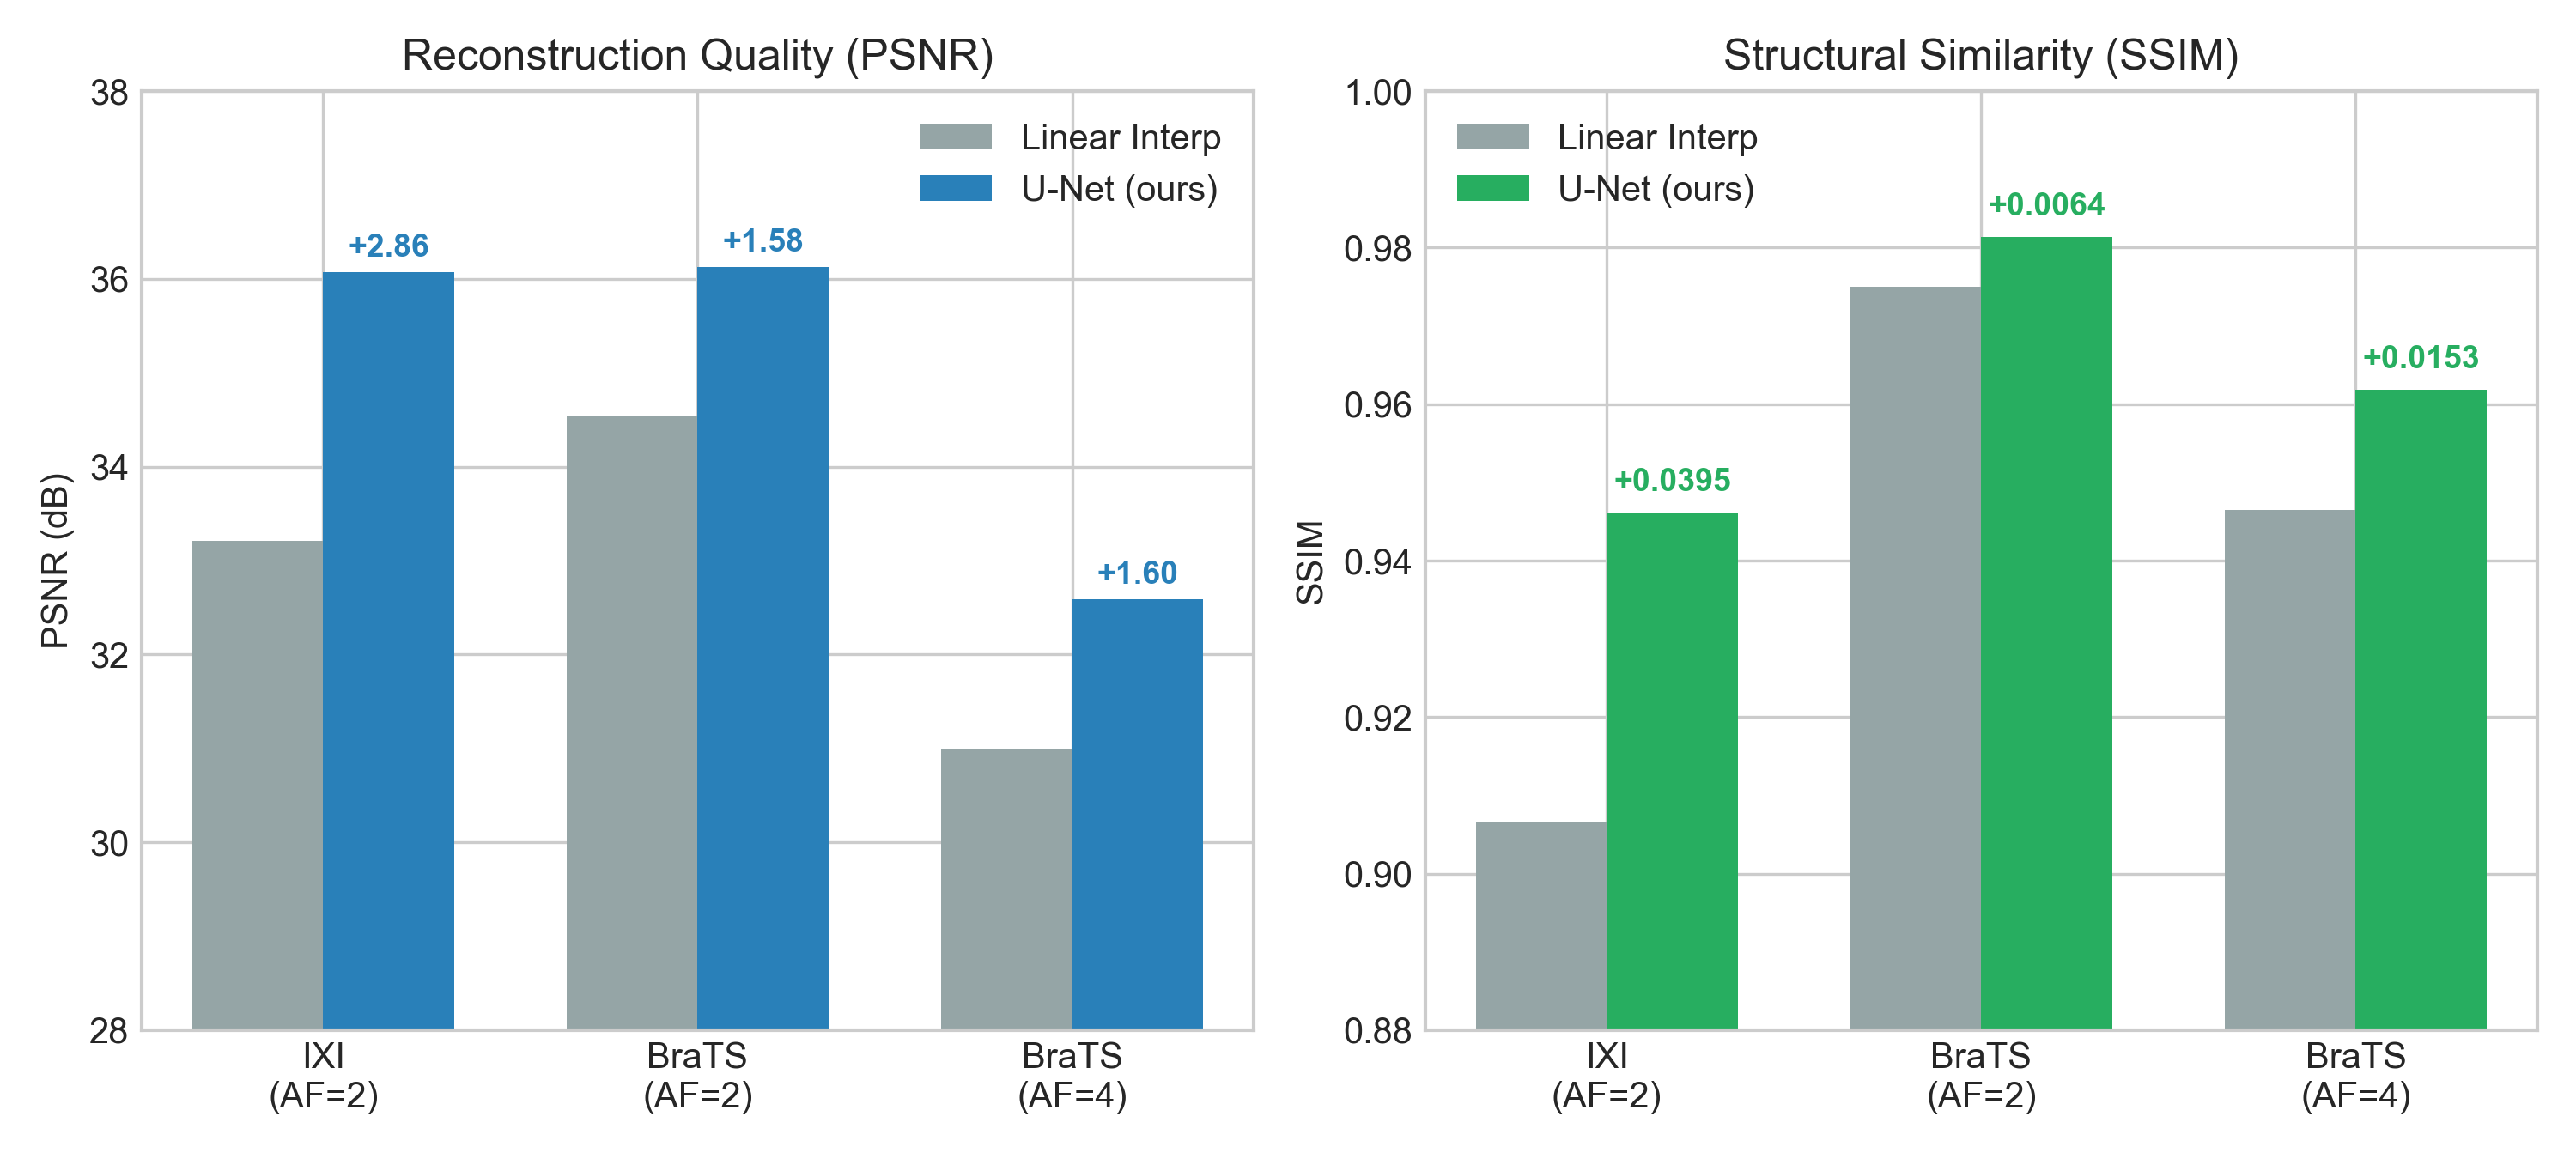
\includegraphics[width=\textwidth]{report_metrics_summary.png}
    \caption{Quantitative reconstruction performance across datasets and acceleration factors. The U-Net consistently outperforms linear interpolation, with the largest structural similarity (SSIM) gains occurring in the harder AF=4 setting.}
    \label{fig:metrics}
\end{figure}

\begin{figure}[htbp]
    \centering
    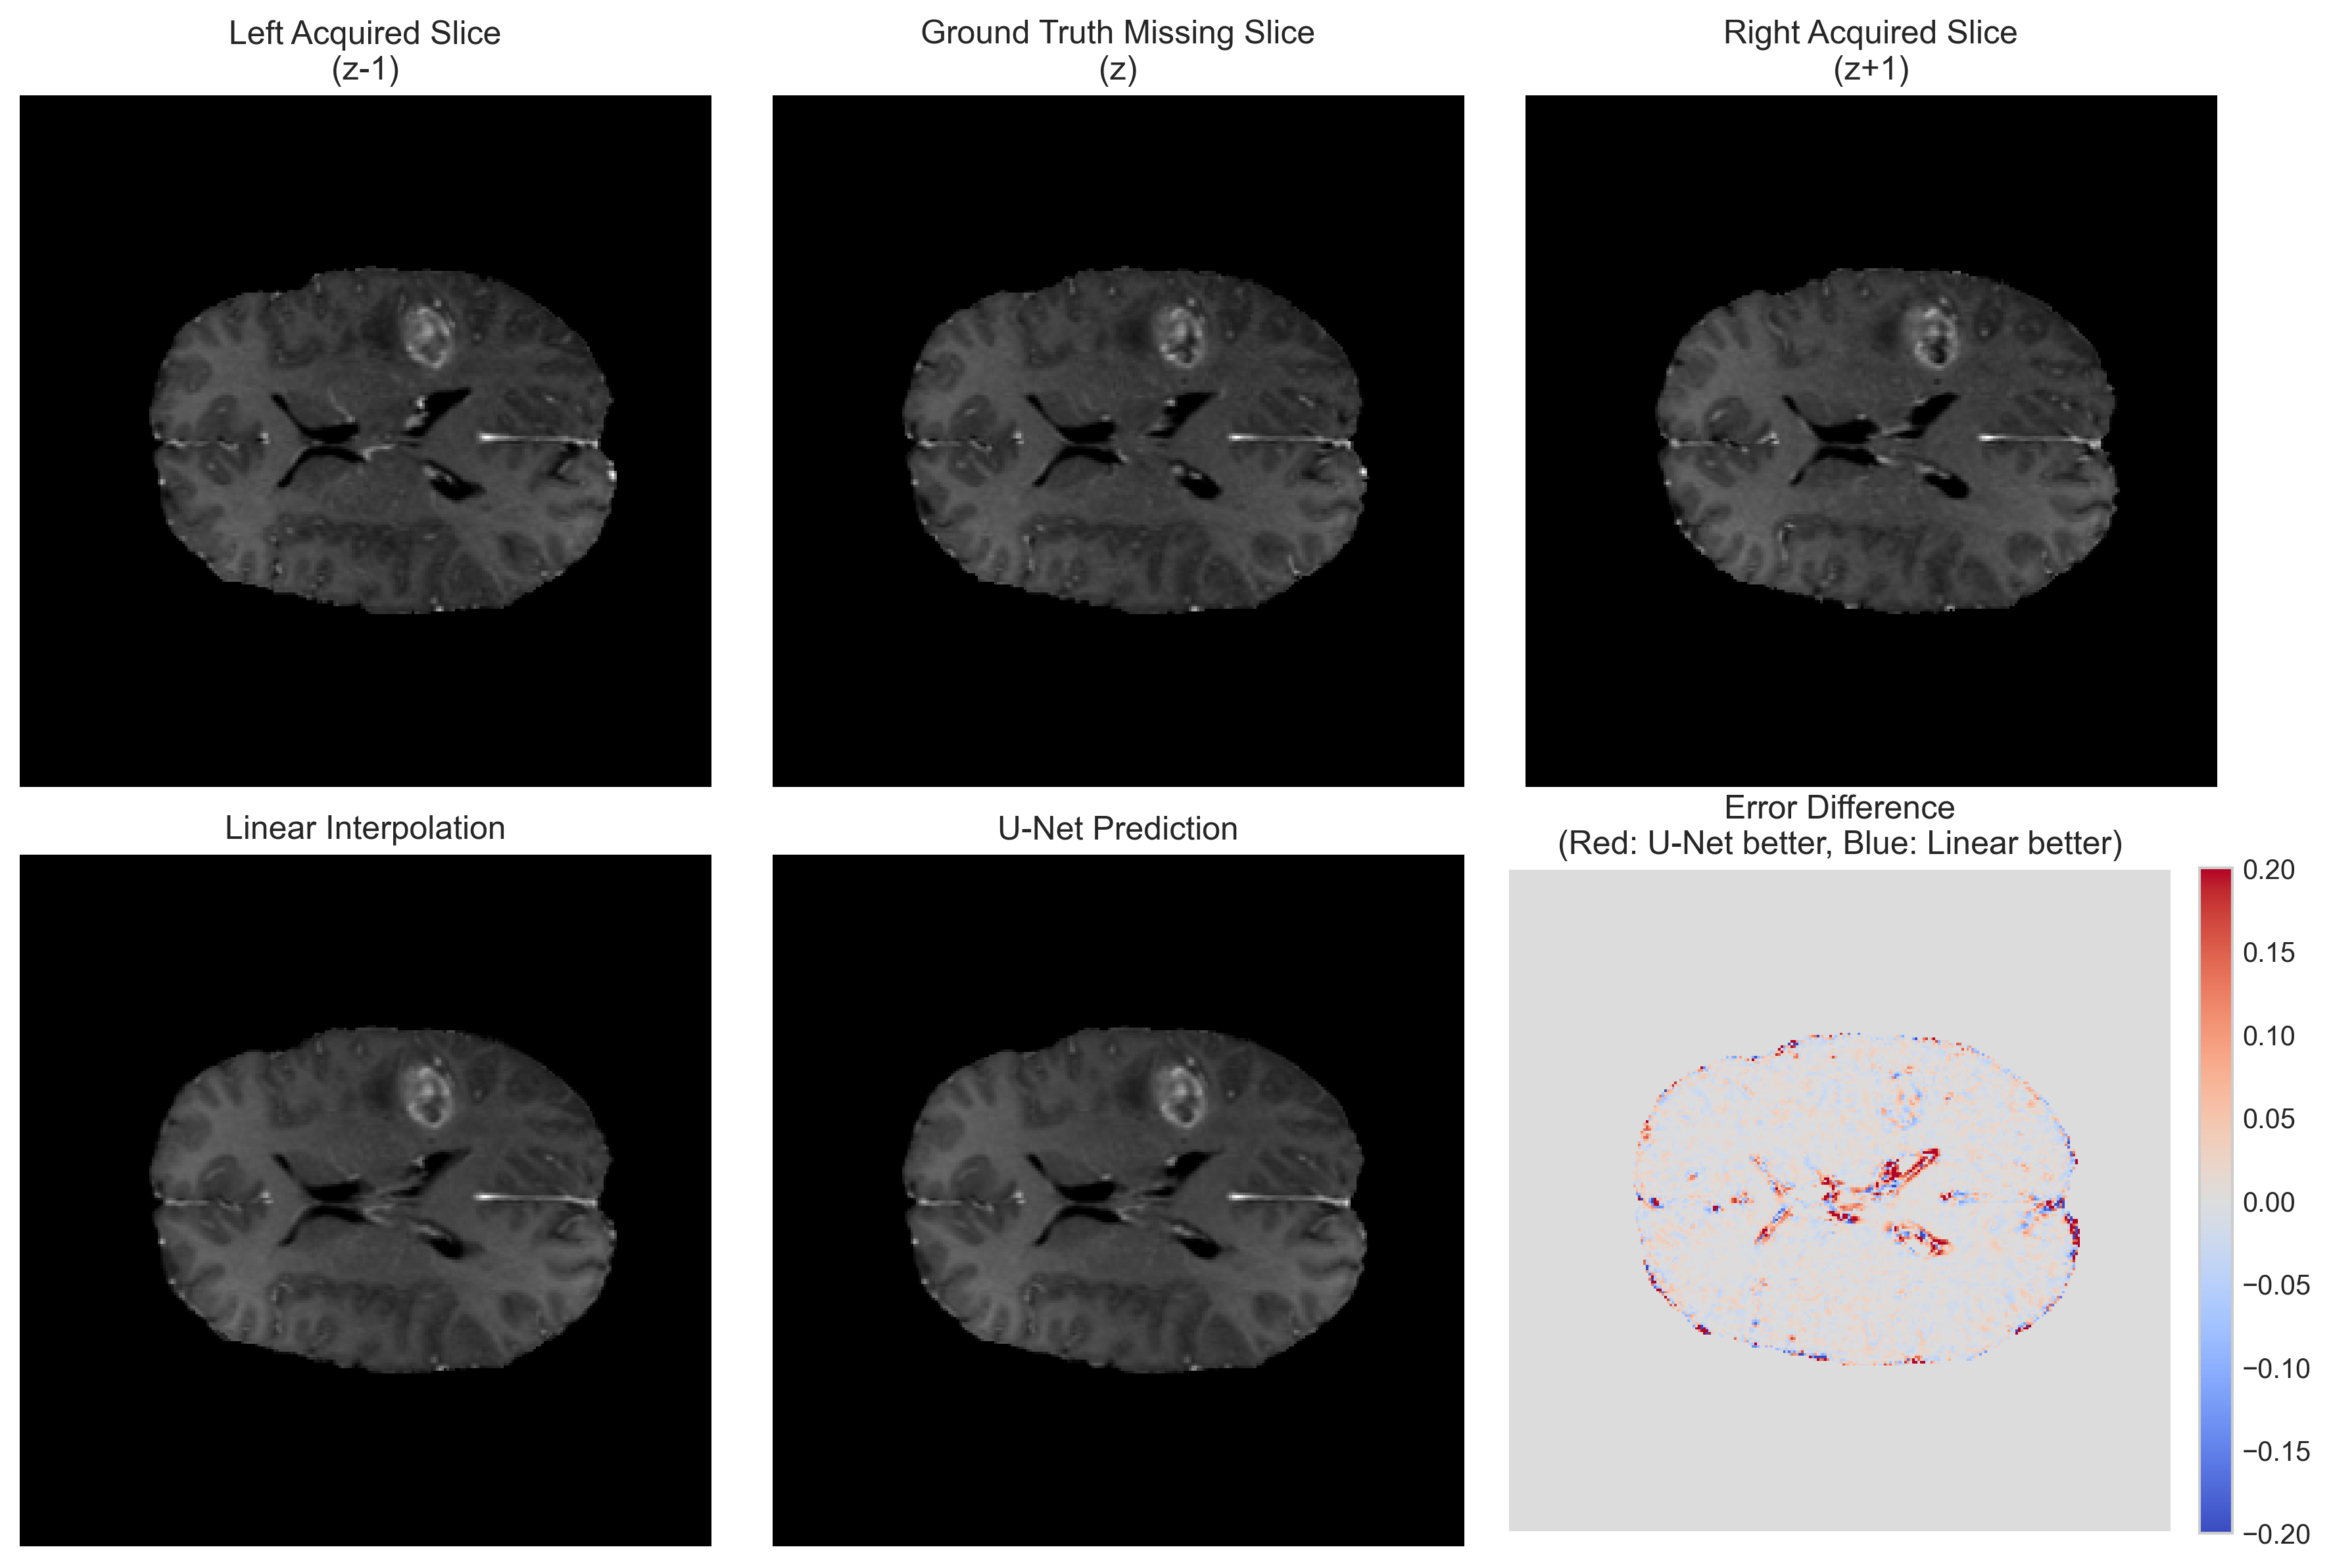
\includegraphics[width=\textwidth]{report_qualitative_sample.png}
    \caption{Qualitative reconstruction of a tumor-containing BraTS slice (AF=2). The error map (bottom right) demonstrates that the U-Net produces significantly lower error (red) around the brain boundary, ventricles, and tumor edges compared to linear interpolation (blue).}
    \label{fig:qualitative}
\end{figure}

\end{document}
